

\documentclass[10pt,twocolumn]{article}

\usepackage[utf8]{inputenc}
\usepackage{times}
\usepackage{mathptmx}  
\usepackage{spverbatim}
\usepackage{graphicx}
\usepackage{float}

\renewcommand {\figurename}{Figur}

\raggedbottom
\sloppy

\title{Laborationsrapport i TSKS10 \emph{Signaler, Information och Kommunikation}}

\author{Peter Keijser Tullstedt \\ pettu298, 940625-0994}

\date{2016-05-12}

\begin{document}

\maketitle

\section{Inledning}

Denna laboration gick ut på att demodulera en smalbandig signal som är I/Q-modulerad
och som har passerat ett delvis okänt filter. Signalen innehåller hörbara signaler i form av 
melodier och ordspråk. För att demodulera signalen behövdes först signalens bärfrekvens tas ut och ekoeffekter hanteras. Laborationens resultat var signalens bärfrekvens $f_c$, ekotidsfördröjningen $\tau_2 - \tau_1$ och en
signal där ordspråk samt melodier kunde höras.\\

Från laborationshandledningen gavs följande information om den givna signalen.
\begin{itemize}

	\item Radiostationen sänder ut en signal med utseendet:
		$x(t) = x_I(t)\cos(2\pi f_c t)-x_Q(t)\sin(2\pi f_c t)+z(t)$,
		där $z(t)$ är signaler ämnade för andra personer.

	\item $x_I(t)$ och $x_Q(t)$ är meddelanden av intresse som innehåller melodi, ordspråk och vitt brus.

	\item Bärfrekvensen $f_c$ är en multipel av 19 kHz.

	\item På grund av ekoeffekter i radioutbredningsmiljön tas följande signal emot:
		$y(t)=x(t - \tau_1)+0,9x(t - \tau_2)$.

	\item Den mottagna signalen lågpassfiltreras och samplas sedan med en samplingsfrekvens $f_s =400 $ 000 Hz.
	
\end{itemize}


\section{Metod}

Laborationen var uppdelad i tre uppgifter; ta reda på bärfrekvensen $f_c$, ta reda på differensen $\tau_2 - \tau_1$ och I/Q-demodulera signalen.

\subsection{Identifiering av bärfrekvens}

Bärfrekvensen fås utifrån amplitudspektrumet för signalen $y(t)$. Figur \ref{ampl} visar amplitudspektrumet $|Y(f)|$. Ur amplitudspektrumet erhålls tre olika bärfrekvenser, genom att titta på de områden som har stor nollskild aktivitet. Eftersom vi vet att den sökta bärfrekvensen är en multipel av 19 kHz kan vi specificera att de möjliga bärfrekvenserna är:

\begin{itemize}

	\item Signal $y_1$ med $f_{c1} = 76$ kHz,
	\item signal $y_2$ med $f_{c2} = 114$ kHz, och
	\item signal $y_3$ med $f_{c3} = 152$ kHz.

\end{itemize}

\begin{figure}[H]
	\centering
	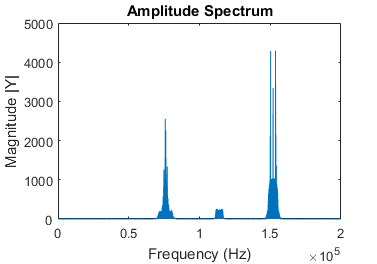
\includegraphics[width=0.4\textwidth]{figures/Figure1.png}
	\caption{Amplitudspektrum till den givna signalen.}
	\label{ampl}
\end{figure}

Signalerna vid de olika frekvenserna filtreras ut med ett bandpassfilter med en bandbredd $B = 20000$, centrerad kring de möjliga bärfrekvenserna.
Figur \ref{filtered} visar de filtrerade signalerna. Signalerna $y_2$ och $y_3$ ser ut att vara brus medan signalen $y_1$ ser ut att ha korrekt innehåll.

\begin{figure}[H]
	\centering
	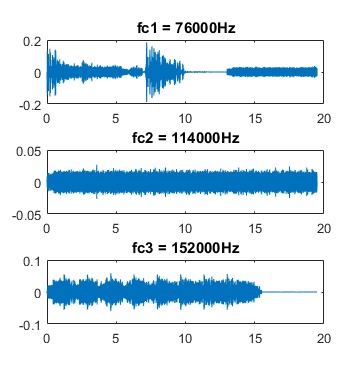
\includegraphics[width=0.3\textwidth]{figures/Figure2.png}
	\caption{Sändarens tre signaler i tidsdomänen. }
	\label{filtered}
\end{figure}

\subsection{Hantering av ekotidsfördröjning}

För att ta bort ekoeffekterna i signalen så behöver ekots tidsfördröjning först hittas. Detta görs genom att autokorrelera signalen $y_1$. Brusliknande signaler ger tydligast resultat vid autokorrelation, så $y_2$ valdes för detta. I Figur \ref{echo} finns en huvudtopp vid $t=0$ och en sidotopp vid $t=0,38$ s. Detta är värdet för tidsfördröjningen $\tau_2 - \tau_1$.


\begin{figure}[H]
	\centering
	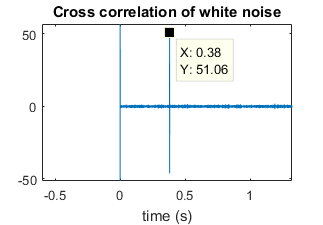
\includegraphics[width=0.3\textwidth]{figures/Figure3.png}
	\caption{Autokorrelation för att bestämma ekots tidsfördröjning.}
	\label{echo}
\end{figure}

Nu kan den ekofria signalen $y'_1(t)$ tas fram från $y_1(t)$. För att ta fram den ekofria signalen används funktionen $y'_1(t)=y_1(t) - 0,9y'_1(t-\tau_2 + \tau_1)$. I MATLAB görs detta genom att i segment av storleken $(\tau_2 - \tau_1) * f_s$

\subsection{IQ-demodulering}

När signalen är ekofri återstår bara I/Q-demodulering innan signalen är färdig. Formeln som används är $x_I(t)=\mathcal{H}^{LP}_{B/2}{2x(t)cos(2\pi f_c t)}$ och $x_Q(t)=-\mathcal{H}^{LP}_{B/2}{2x(t)sin(2\pi f_c t)}$. I detta fall är $x(t)=y'_1(t)$, $f_c = f_{c1} = 74000$ Hz och $B=20000$ Hz. Basbandsignalerna $x_I$ och $x_Q$ kan nu spelas upp med hörbart ljud.

\section{Resultat}

Den sökta informationen är:
\begin{itemize}
\item Bärfrekvensen för nyttosignalen är $f_c=76$ kHz,
\item ekots tidsfördröjning $\tau_2 - \tau_1 = 0,38$ s, 
\item ordspråket i I-signalen är: "Inget ont som inte har något gott med sig" och
\item ordspråket i Q-signalen är: "Väck inte den björn som sover".
\end{itemize}

\onecolumn
\clearpage

\section*{Min Matlab-kod:}

\begin{spverbatim}

clc;clear; close all;

%data in y, sample rate in Fs
[y, Fs] = audioread('signal-pettu298.wav');

% Transform
Y = fft(y);

% Check carrier frequencies
len = length(y);
freqAxis = Fs/2 * linspace(0, 1, len/2);


plot(freqAxis, abs(Y(1:len/2)));
title('Amplitude Spectrum');
xlabel('Frequency (Hz)');
ylabel('Magnitude |Y|');

% Filter the appropriate values, can be seen in Amplitude Spectrum. 
bandwidth = 20000;     % Set the bandwidth of filters to 2*10^4 Hz.
   
% Frequencies found in Amplitude Spectrum. Multiples of 19 kHz.
fc1 = 76000;
fc2 = 114000;
fc3 = 152000;

% Generate vector with len evenly spaced points
timeAxis = linspace(0, len / Fs, len)';    

% Butterworth-filter the found frequencies.
[B, A] = butter(10, [fc1 - bandwidth/2, fc1 + bandwidth/2]/(Fs/2));
y1 = filter(B, A, y);

[B, A] = butter(10, [fc2 - bandwidth/2, fc2 + bandwidth/2]/(Fs/2));
y2 = filter(B, A, y);

[B, A] = butter(10, [fc3 - bandwidth/2, fc3 + bandwidth/2]/(Fs/2));
y3 = filter(B, A, y);

% Plot the filtered signals.
figure(2);
subplot(3,1,1);
plot(timeAxis, y1);
title(['fc1 = ' num2str(fc1) 'Hz']);

subplot(3,1,2);
plot(timeAxis, y2);
title(['fc2 = ' num2str(fc2) 'Hz']);

subplot(3,1,3);
plot(timeAxis, y3);
title(['fc3 = ' num2str(fc3) 'Hz']);

% y1 (76 kHz) seems to be the desired signal.
% y2 (114 kHz) seems to be white noise.

% Cross-correlation of white noise (y2) to find echo time delay. 
[corr, lags] = xcorr(y2);
corr = corr(lags > 0); % Only positive time is relevant.
lags = lags(lags > 0);

% Plot Cross-correlation of white noise.
figure(3);
subplot(1,1,1);
plot(lags/Fs, corr);
xlabel('time (s)');
title('Cross correlation of white noise');

tau_2 = 0.38;     % Difference in seconds from correlation plot.
nrSamples = tau_2 * Fs;    % Difference in samples.

% Echo Cancellation.
y1NoEcho = zeros(size(y1));

% Add echo-free first segment to y1NoEcho. 
y1NoEcho(1:nrSamples) = y1(1:nrSamples);

% Split Echo Cancellation into segments of size nrSamples.
for i = 1:46

    % Segment nrSamples*i : nrSamples + nrSamples*i of y1NoEcho.
    segNoEcho = y1NoEcho((1 + nrSamples*i):(nrSamples + nrSamples*i));  

    % Following Segment but in signal y1.
    segOriginal = y1((nrSamples + 1 + nrSamples*i):(i+2)*nrSamples);          
    
    % Set segment from segOriginal in y1NoEcho.
    y1NoEcho((nrSamples + 1 + nrSamples*i):(i+2)*nrSamples) 
    							= segOriginal - 0.9*segNoEcho;  

end

% Filter for IQ-demodulation.
[B,A] = butter(8, bandwidth/(Fs/2), 'low');

% I- and Q Carrier Signals. 
ic = 2*cos(2*pi*fc1*timeAxis);
qc = -2*sin(2*pi*fc1*timeAxis);

% Filter I and Q components of signal y1NoEcho.
yi = filter(B, A, y1NoEcho.*ic);
yq = filter(B, A, y1NoEcho.*qc);

i = decimate(yi, 10);
q = decimate(yq, 10);

% Play sound.
soundsc(i, Fs/10);  % "Inget ont som inte har något gott med sig".
pause;
soundsc(q, Fs/10);  % "Väck inte den björn som sover".


\end{spverbatim}

\end{document}
